\documentclass[aspectratio=43,17pt]{beamer} % or 14 or 17 or 20

\usepackage{tikz,pgf,lmodern,textpos,hyperref,graphicx,booktabs,appendixnumberbeamer,cleveref,fancybox,multicol}
\usepackage{pgfcalendar,svg,subfiles,chronosys,cancel,xcolor,color,nth,datenumber,xparse,fp,stackengine,makecell}
\usepackage{enumitem,setspace}
\usepackage{marvosym} % \MVRIGHTarrow
\usepackage{amsmath}
\usepackage{centernot}
\usetikzlibrary{positioning}
\usepackage[outline]{contour}
\usepackage[citestyle=authoryear-comp,backend=bibtex]{biblatex}
\usepackage[export]{adjustbox}
\usepackage[en-US]{datetime2}
\usepackage[normalem]{ulem}
\bibliography{references}
\usetheme[numbering=none]{metropolis}

\setlist[itemize]{label={--}}
% \setlist[itemize]{leftmargin=*}

% \bibliography{references}

%!TEX Root = ./presentation.tex

\definecolor{Blue}{HTML}{00548f}
\definecolor{Cardinal Red}{HTML}{8c1515}
\definecolor{White}{HTML}{ffffff}
\definecolor{Cool Grey}{HTML}{4d4f53}
\definecolor{Black}{HTML}{2e2d29}
\definecolor{Bright Red}{HTML}{B1040E}
\definecolor{Dark Red}{HTML}{820000}
\definecolor{Chocolate}{HTML}{2F2424}
\definecolor{Stone}{HTML}{544948}
\definecolor{Fog}{HTML}{F4F4F4}
\definecolor{Light Sandstone}{HTML}{F9F6EF}
\definecolor{Sandstone}{HTML}{d2c295}
\definecolor{Warm Grey}{HTML}{3f3c30}
\definecolor{Beige}{HTML}{9d9573}
\definecolor{Light Sage}{HTML}{c7d1c5}
\definecolor{Clay}{HTML}{5f574f}
\definecolor{Cloud}{HTML}{dad7cb}
\definecolor{Driftwood}{HTML}{b6b1a9}
\definecolor{Stone}{HTML}{928b81}
\definecolor{Sandhill}{HTML}{b3995d}
\definecolor{Palo Alto}{HTML}{175e54}
\definecolor{Teal}{HTML}{00505c}
\definecolor{Purple}{HTML}{53284f}
\definecolor{Redwood}{HTML}{8d3c1e}
\definecolor{Brown}{HTML}{5e3032}
\definecolor{Sky}{HTML}{0098db}
\definecolor{Lagunita}{HTML}{007c92}
\definecolor{Mint}{HTML}{009b76}
\definecolor{Gold}{HTML}{b26f16}
\definecolor{Sun}{HTML}{eaab00}
\definecolor{Poppy}{HTML}{e98300}

\definecolor{USF Green}{HTML}{00543C}
\definecolor{USF Gold}{HTML}{FDBB30}
\definecolor{USF Grey}{HTML}{919194}
% \definecolor{USF }{HTML}{e98300}


\setbeamercolor{normal text}{fg=Black,bg=White}
\hypersetup{colorlinks,linkcolor=USF Green,urlcolor=USF Green,citecolor=USF Green}
% \setbeamercolor{frametitle}{bg=Cardinal Red, fg=Blue}


\setbeamercolor{palette primary}{bg=Fog, fg=USF Green}
\setbeamercolor{palette secondary}{bg=USF Green, fg=Fog}
\setbeamercolor{frametitle}{bg=Fog,fg=USF Green}

% \setbeamercolor{section title}{fg=Dark Red, bg=Fog}
\setbeamercolor{alerted text}{fg=USF Green}

\newcommand{\soutthick}[1]{%
    \renewcommand{\ULthickness}{2.4pt}%
       \sout{#1}%
    \renewcommand{\ULthickness}{.4pt}% Resetting to ulem default
}


  \setbeamercolor{normal text}{%
    fg=Cool Grey,
    bg=White
  }

\setbeamercolor{palette primary}{fg=Fog, bg=Dark Red}
\setbeamercolor{palette secondary}{bg=Dark Red, bg=Fog}
\setbeamercovered{transparent}
% \setbeamercolor{background canvas}{bg=Fog}
\setbeamercolor{frametitle}{bg=Dark Red,fg=Fog}
\hypersetup{colorlinks,linkcolor=Blue,urlcolor=Blue,citecolor=Blue}
\setbeamercolor{alerted text}{fg=Bright Red}
\setbeamertemplate{caption}{\insertcaption}


\setsansfont[BoldFont={Source Sans Pro Bold},
              Numbers={OldStyle}]{Source Sans Pro}
\setmainfont[BoldFont={Source Serif Pro Semibold},
              Numbers={OldStyle}]{Source Serif Pro}
\setmonofont{Source Code Pro}


\metroset{titleformat=smallcaps,numbering=none}


\newenvironment{mystepwiseitemize}{\begin{itemize}[<+-| alert@+>]}{\end{itemize}}



\setlist{nosep}

\title{Data Ethics Lecture 6}
\subtitle{Organizing and Activism}
\author[Ali Alkhatib]{{Ali Alkhatib}\\
\href{http://twitter.com/_alialkhatib}{@\_alialkhatib} || \href{mailto:hi@al2.in}{hi@al2.in}}
\date{March April 14, 2022}

% \date{\today}


\newcommand{\onlyinsubfile}[1]{#1}
\newcommand{\notinsubfile}[1]{}

\begin{document}
\renewcommand{\onlyinsubfile}[1]{}
\renewcommand{\notinsubfile}[1]{#1}


\begin{frame}
\titlepage
\end{frame}

\begin{frame}\frametitle{Roadmap for today}
\begin{columns}
\begin{column}{0.5\textwidth}
Lectures 3-4(/5) \hfill \MVRightarrow{}

\vspace{2em}

Course survey \hfill \MVRightarrow{}
\end{column}
\begin{column}{0.4\textwidth}
{\small ~ \vspace{0.5em} links on canvas(?)}

\vspace{2em}

{\small links here \& on canvas(?)}
\end{column}
\end{columns}

\vspace{2em}

\strong{Organizing and Activism}


\end{frame}


\begin{frame}{class survey}
\begin{columns}
\begin{column}{0.3\textwidth}
{Please fill this out if you can! \MVRightarrow{}}
\end{column}
\begin{column}{0.4\textwidth}
\hspace*{-3em}\includegraphics[width=1.5\textwidth]{figures/survey.png}
\end{column}
\end{columns}

\end{frame}

\section{Organizing}

\begin{frame}[standout]
    
A dilemma!

\end{frame}


\begin{frame}[plain]
    
    \centering

\visible<+->{You're working with a dataset that\alt<-5>{\dots}{}}

\only<-5>{\begin{columns}
\begin{column}{0.33\textwidth}

\temporal<+-4>{\visible<0>{\includegraphics[width=\textwidth]{figures/news/worldcoin.png}}}{\includegraphics[width=\textwidth]{figures/news/worldcoin.png}}{\includegraphics[width=\textwidth]{figures/news/worldcoin_grayed.png}}

\end{column}
\begin{column}{0.33\textwidth}

\temporal<+-4>{}{\includegraphics[width=\textwidth]{figures/news/tracker3.png}}{\includegraphics[width=\textwidth]{figures/news/tracker3_grayed.png}}

\end{column}
\begin{column}{0.33\textwidth}

\temporal<+-4>{}{\includegraphics[width=\textwidth]{figures/news/nytMentalHealth.png}}{\includegraphics[width=\textwidth]{figures/news/nytMentalHealth_grayed.png}}


\end{column}
\end{columns}}

\only<6>{

was collected \strong{deceptively} or dishonestly

\strong{disempowers} people

\strong{marginalizes} or oppresses people
}

\end{frame}




\begin{frame}{what to do?}
    
should you\dots

  \begin{itemize}
    \item<+-> talk to your manager?
    \item<+-> leave?
    \item<+-> organize with others?
  \end{itemize}


\centering
\visible<+->{there are good reasons for any of these}


\end{frame}

\section{working with management}

\begin{frame}[plain]

\only<+>{If you can find ways to align \strong{ethical values}
with
\strong{business incentives} (including {regulatory incentives}),
this might work!}

\only<+>{}

\end{frame}


\section{leave?}

\begin{frame}[plain]

Can you meaningfully \strong{reduce harm}?

\hfill\dots or are you \strong{perpetuating harm}?

\vspace{2em}

Do you have a \strong{theory of change}?


\end{frame}




\section{organizing with others}

\begin{frame}{success stories}
    
There are plenty of success stories to draw inspiration and lessons from

\begin{itemize}
  \item community organizing
  \item workplace organizing
\end{itemize}

\end{frame}


\begin{frame}{community organizing}

\begin{columns}
\begin{column}{0.33\textwidth}

\visible<+->{
\hspace*{-1.5em}
\includegraphics[width=2\textwidth]{figures/news/SD.png}}

\end{column}
\begin{column}{0.33\textwidth}

\visible<+->{
\hspace*{-2.5em}
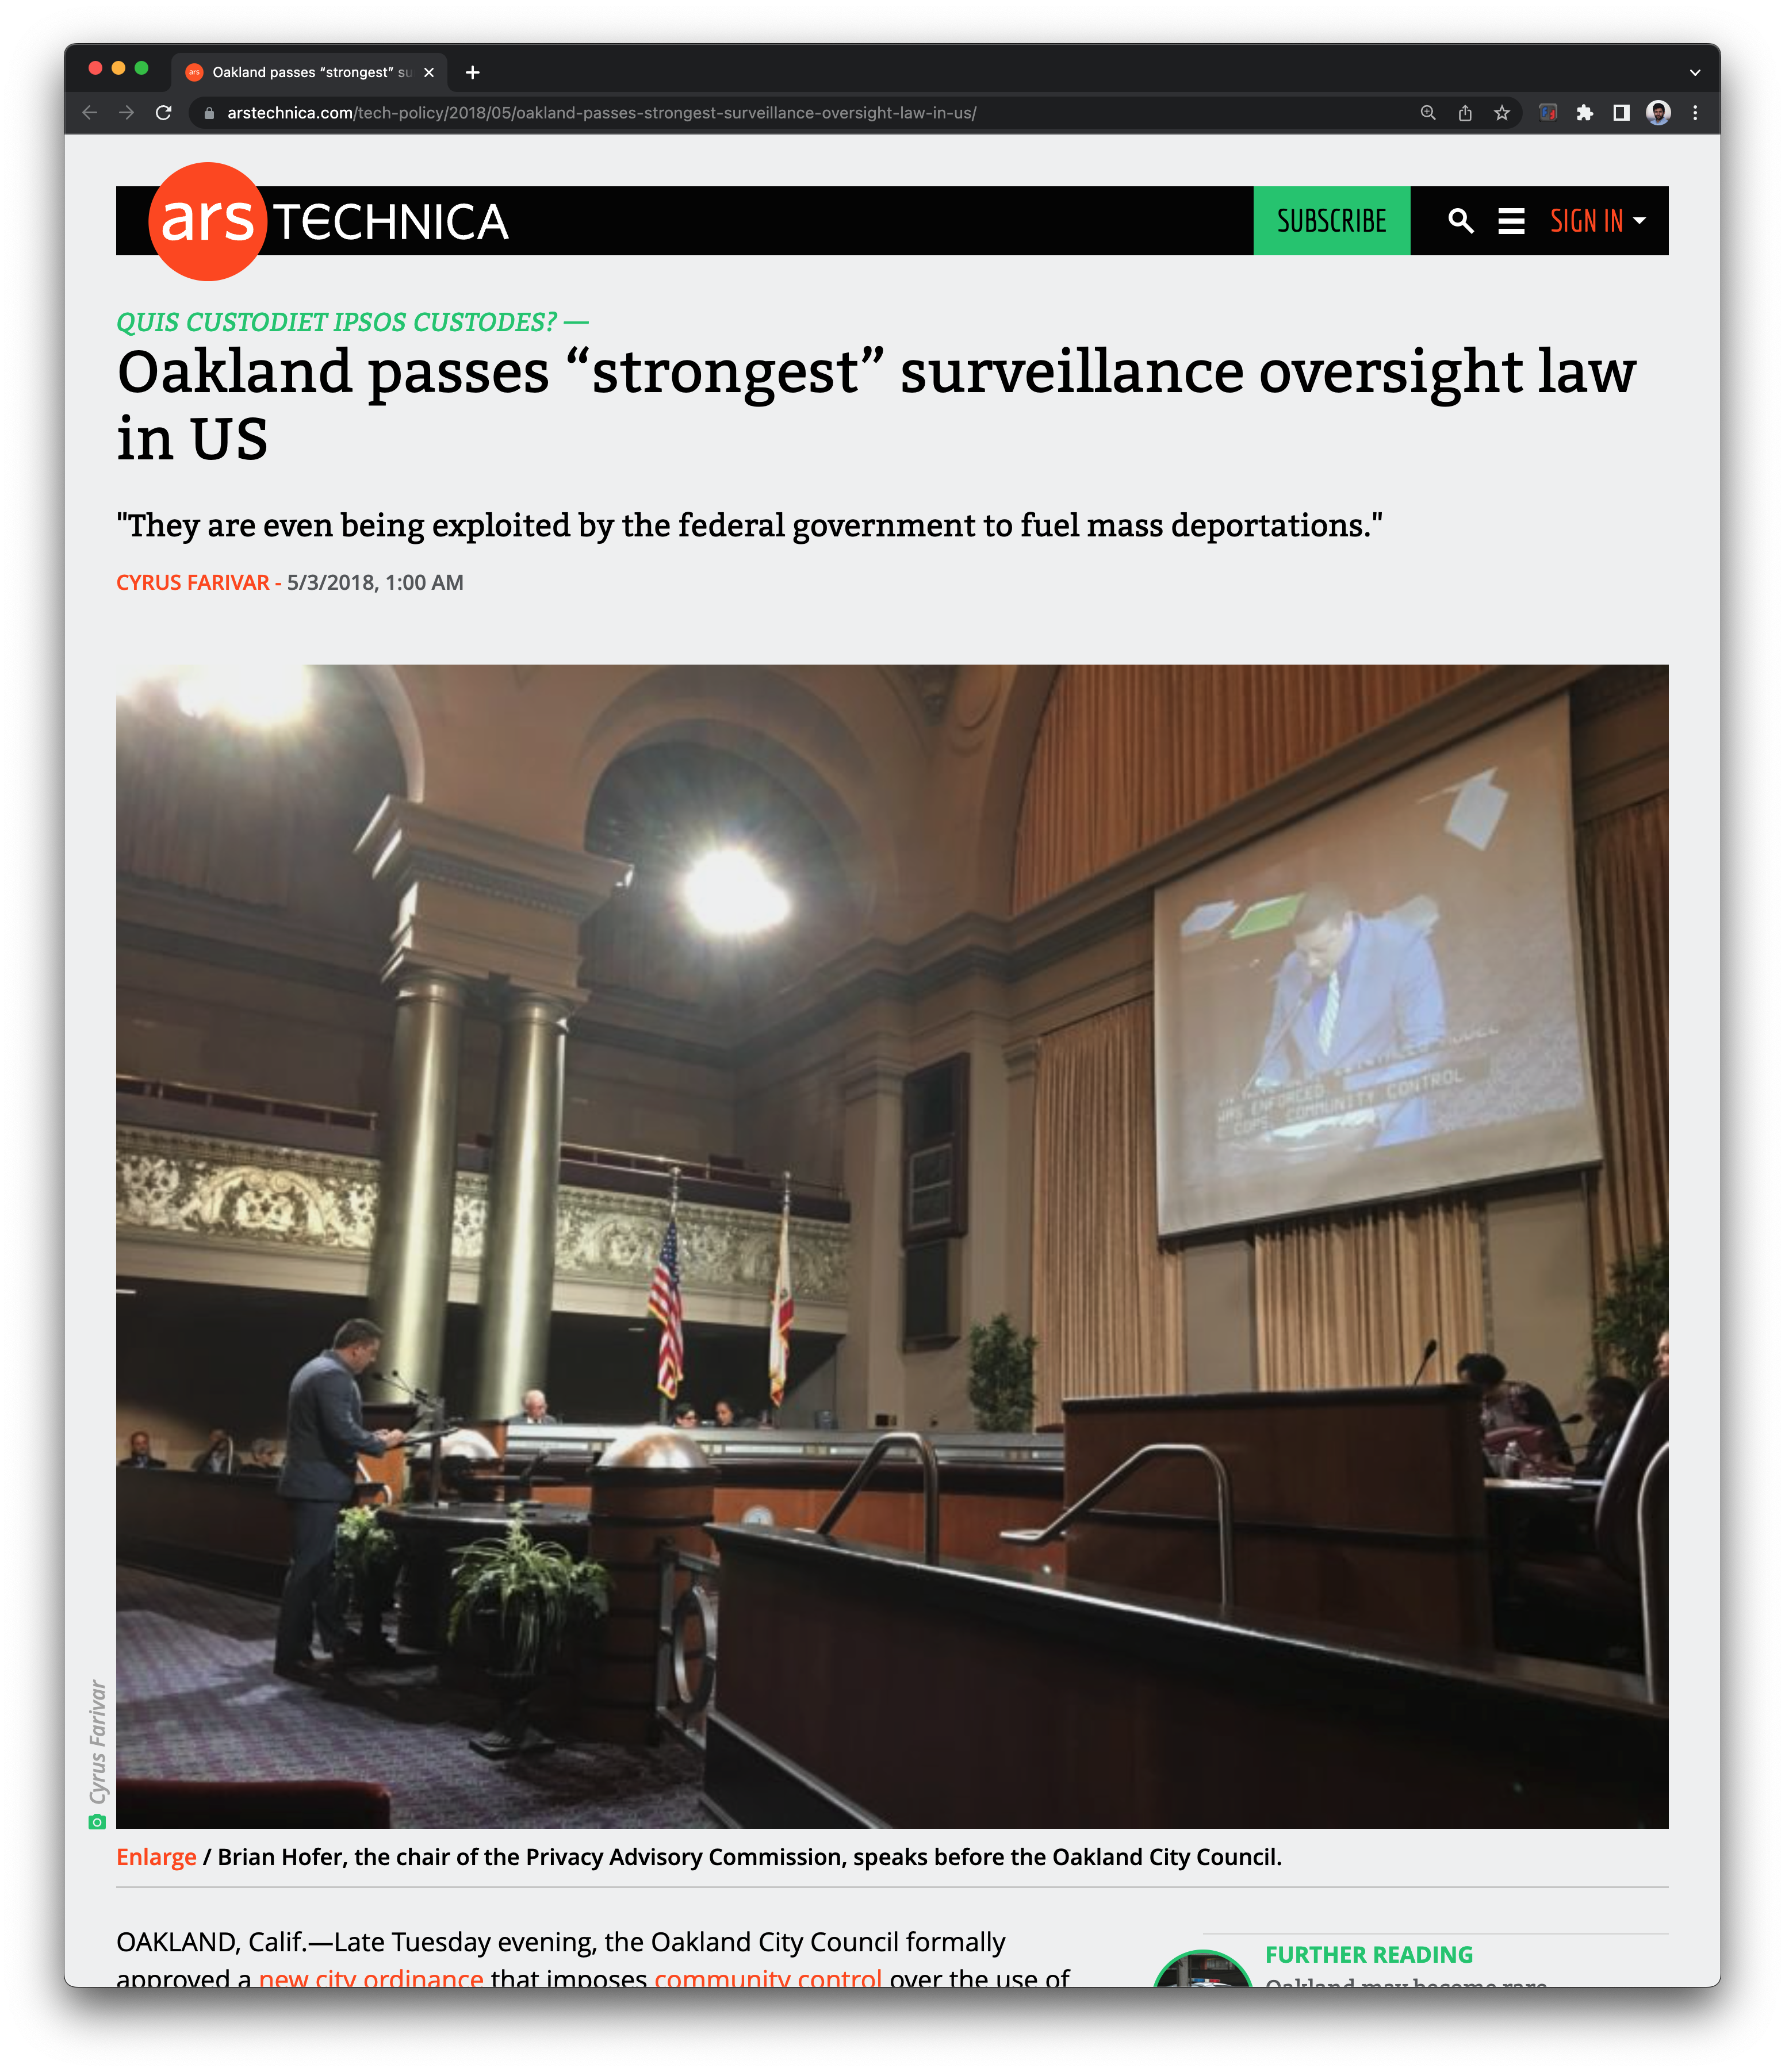
\includegraphics[width=2\textwidth]{figures/news/OAK.png}}

\end{column}
\begin{column}{0.33\textwidth}


\visible<+->{
\hspace*{-2.5em}
\includegraphics[width=2\textwidth]{figures/news/BOS.png}}

\end{column}
\end{columns}

\end{frame}



\begin{frame}{what can we learn?}
    
\begin{itemize}
  \item<+-> \alt<.>{\strong{listen}}{listen} to people living there
  \item<+-> identify when it's best to \alt<.>{\strong{speak}}{speak} vs \alt<.>{\strong{boost}}{boost} others' voices
  \item<+-> \alt<.>{\strong{amplify}}{amplify} and \alt<.>{\strong{support}}{support} their voices
\end{itemize}

\end{frame}


\begin{frame}[plain,label=newsythings]
    \centering


\begin{figure}
\vspace*{-2.25em}

\only<+>{\hspace*{-2.75em}\includegraphics[width=1.3\textwidth]{figures/news/twc_2.png}}

\only<+>{\hspace*{-2.75em}\includegraphics[width=1.3\textwidth]{figures/news/balance_2.png}}

\only<+>{\hspace*{-2.75em}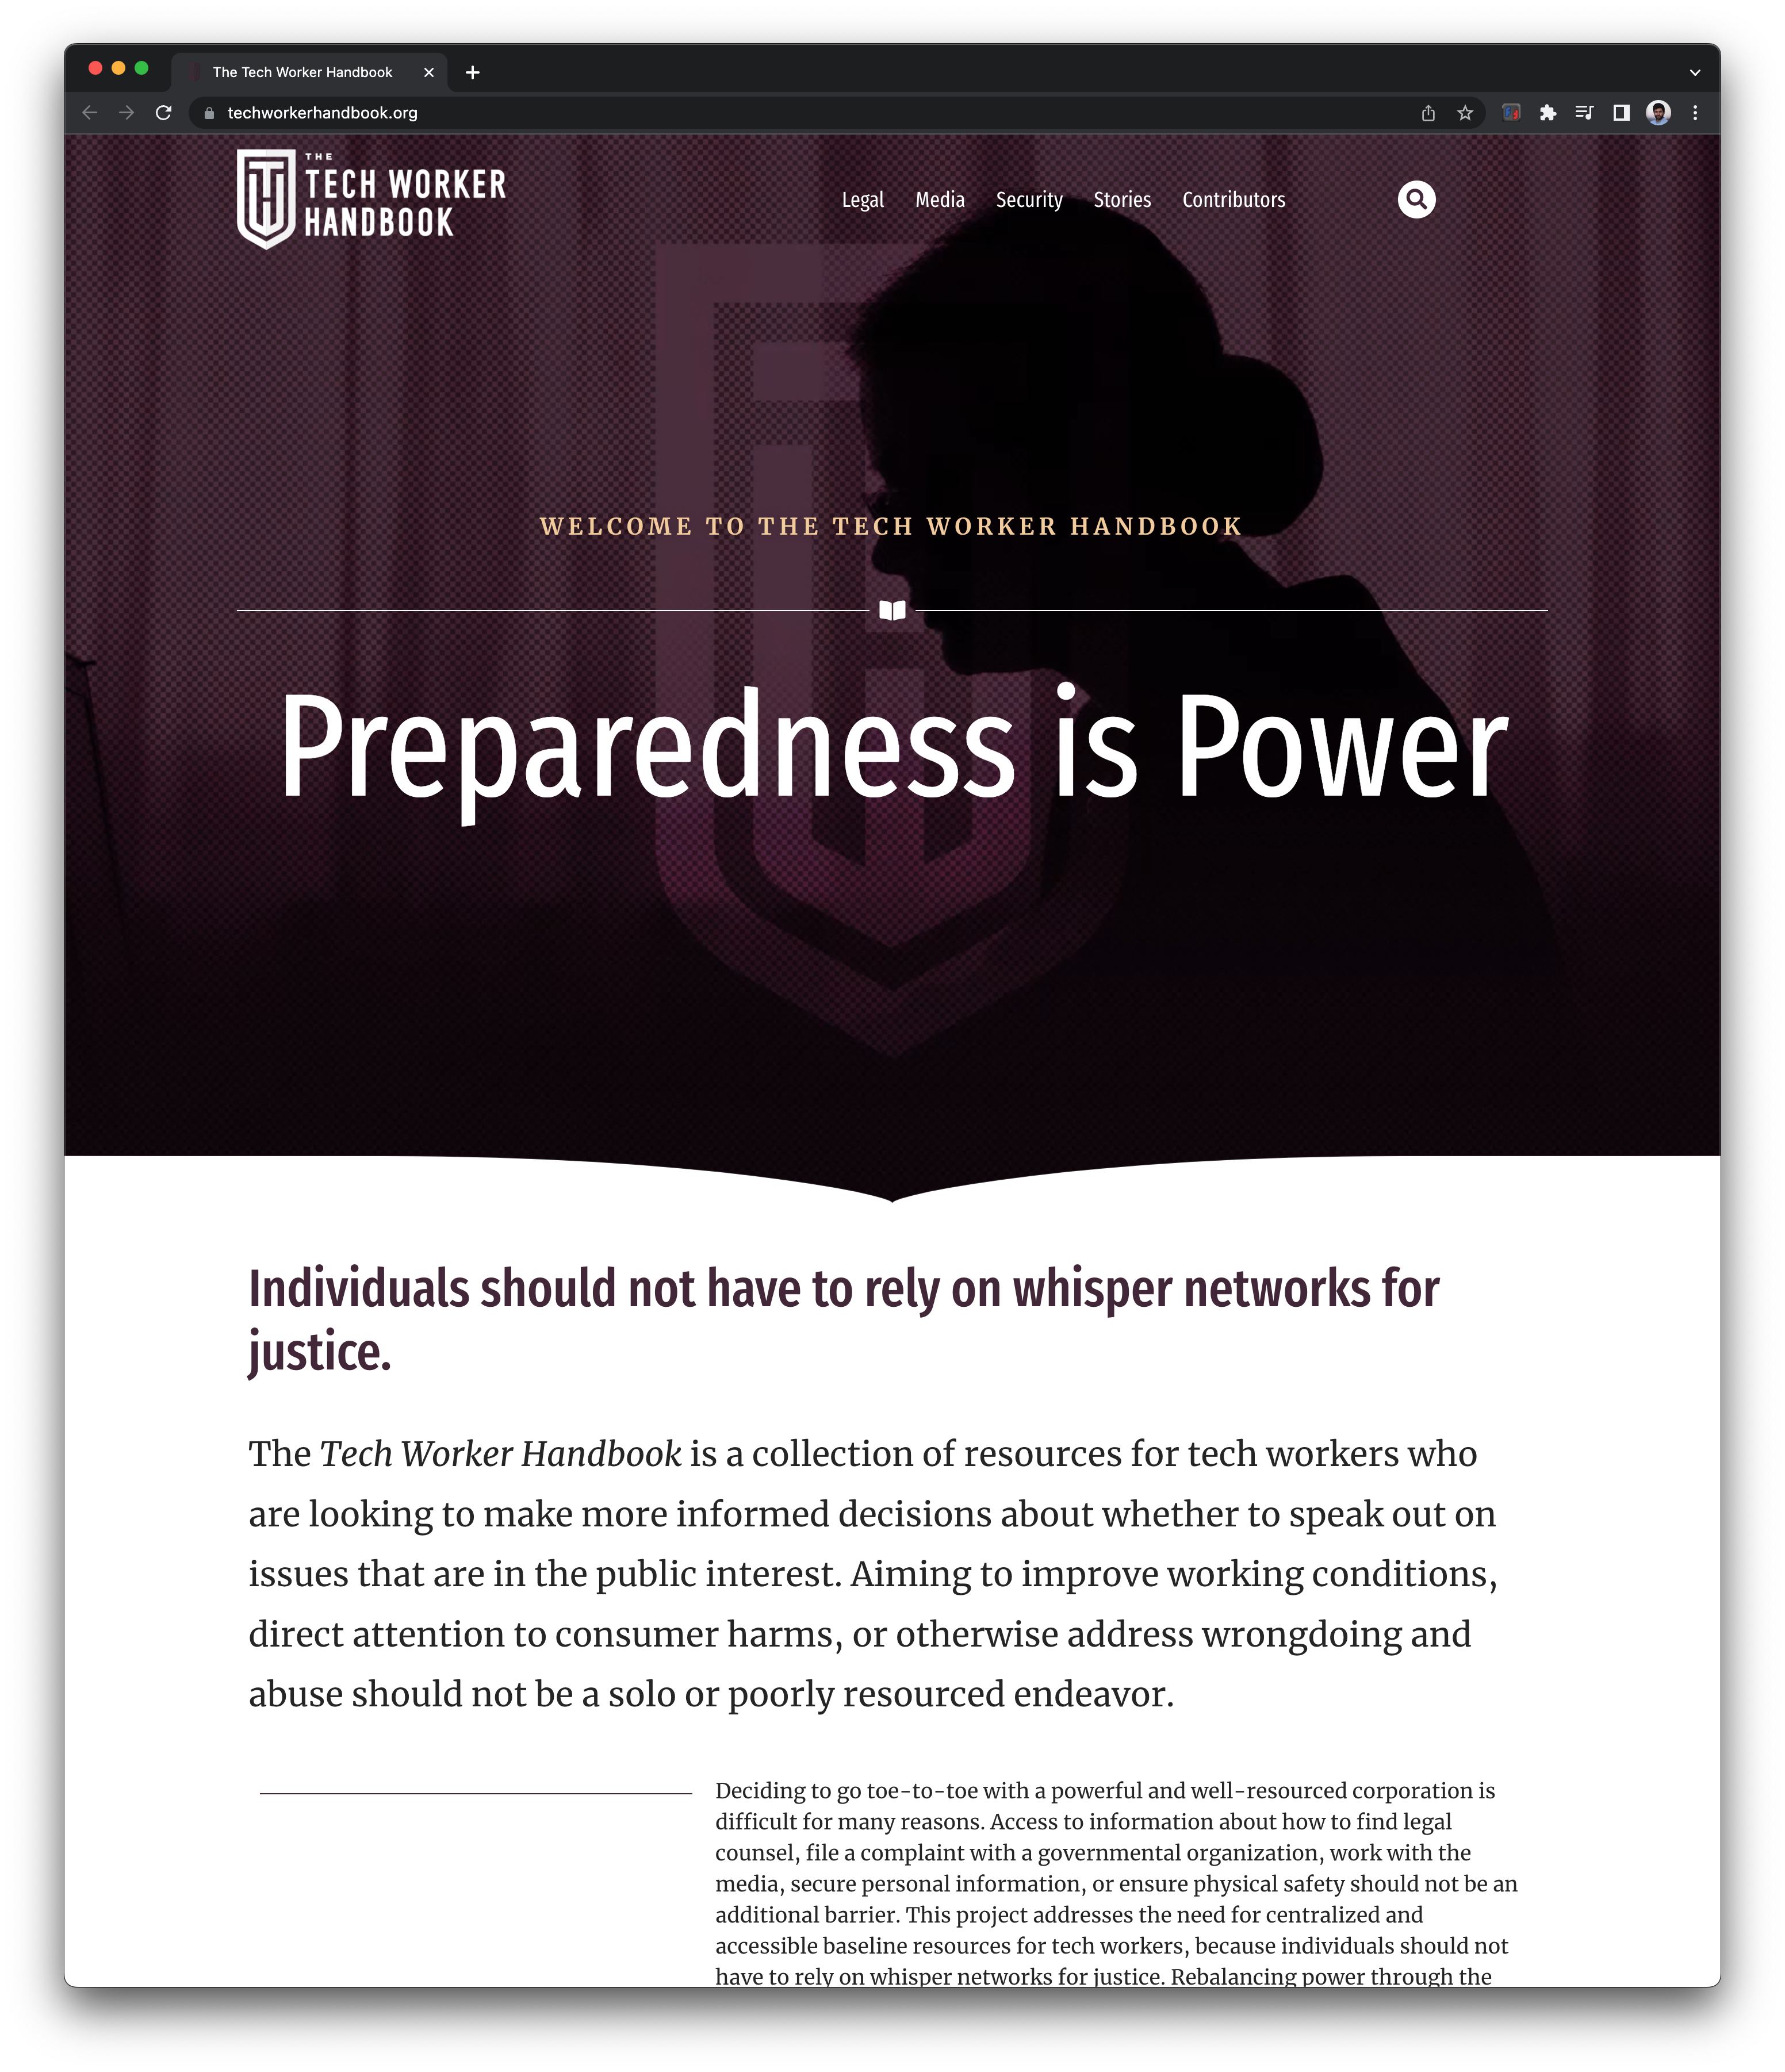
\includegraphics[width=1.3\textwidth]{figures/news/twh_2.png}}

\end{figure}
\end{frame}


\begin{frame}[plain]

\begin{columns}
\begin{column}{0.33\textwidth}

\hspace*{-1.5em}
\includegraphics[width=1.5\textwidth]{figures/news/twc_2.png}

\end{column}
\begin{column}{0.33\textwidth}

\hspace*{-1.5em}
\includegraphics[width=1.5\textwidth]{figures/news/balance_2.png}

\end{column}
\begin{column}{0.33\textwidth}

\hspace*{-1.5em}
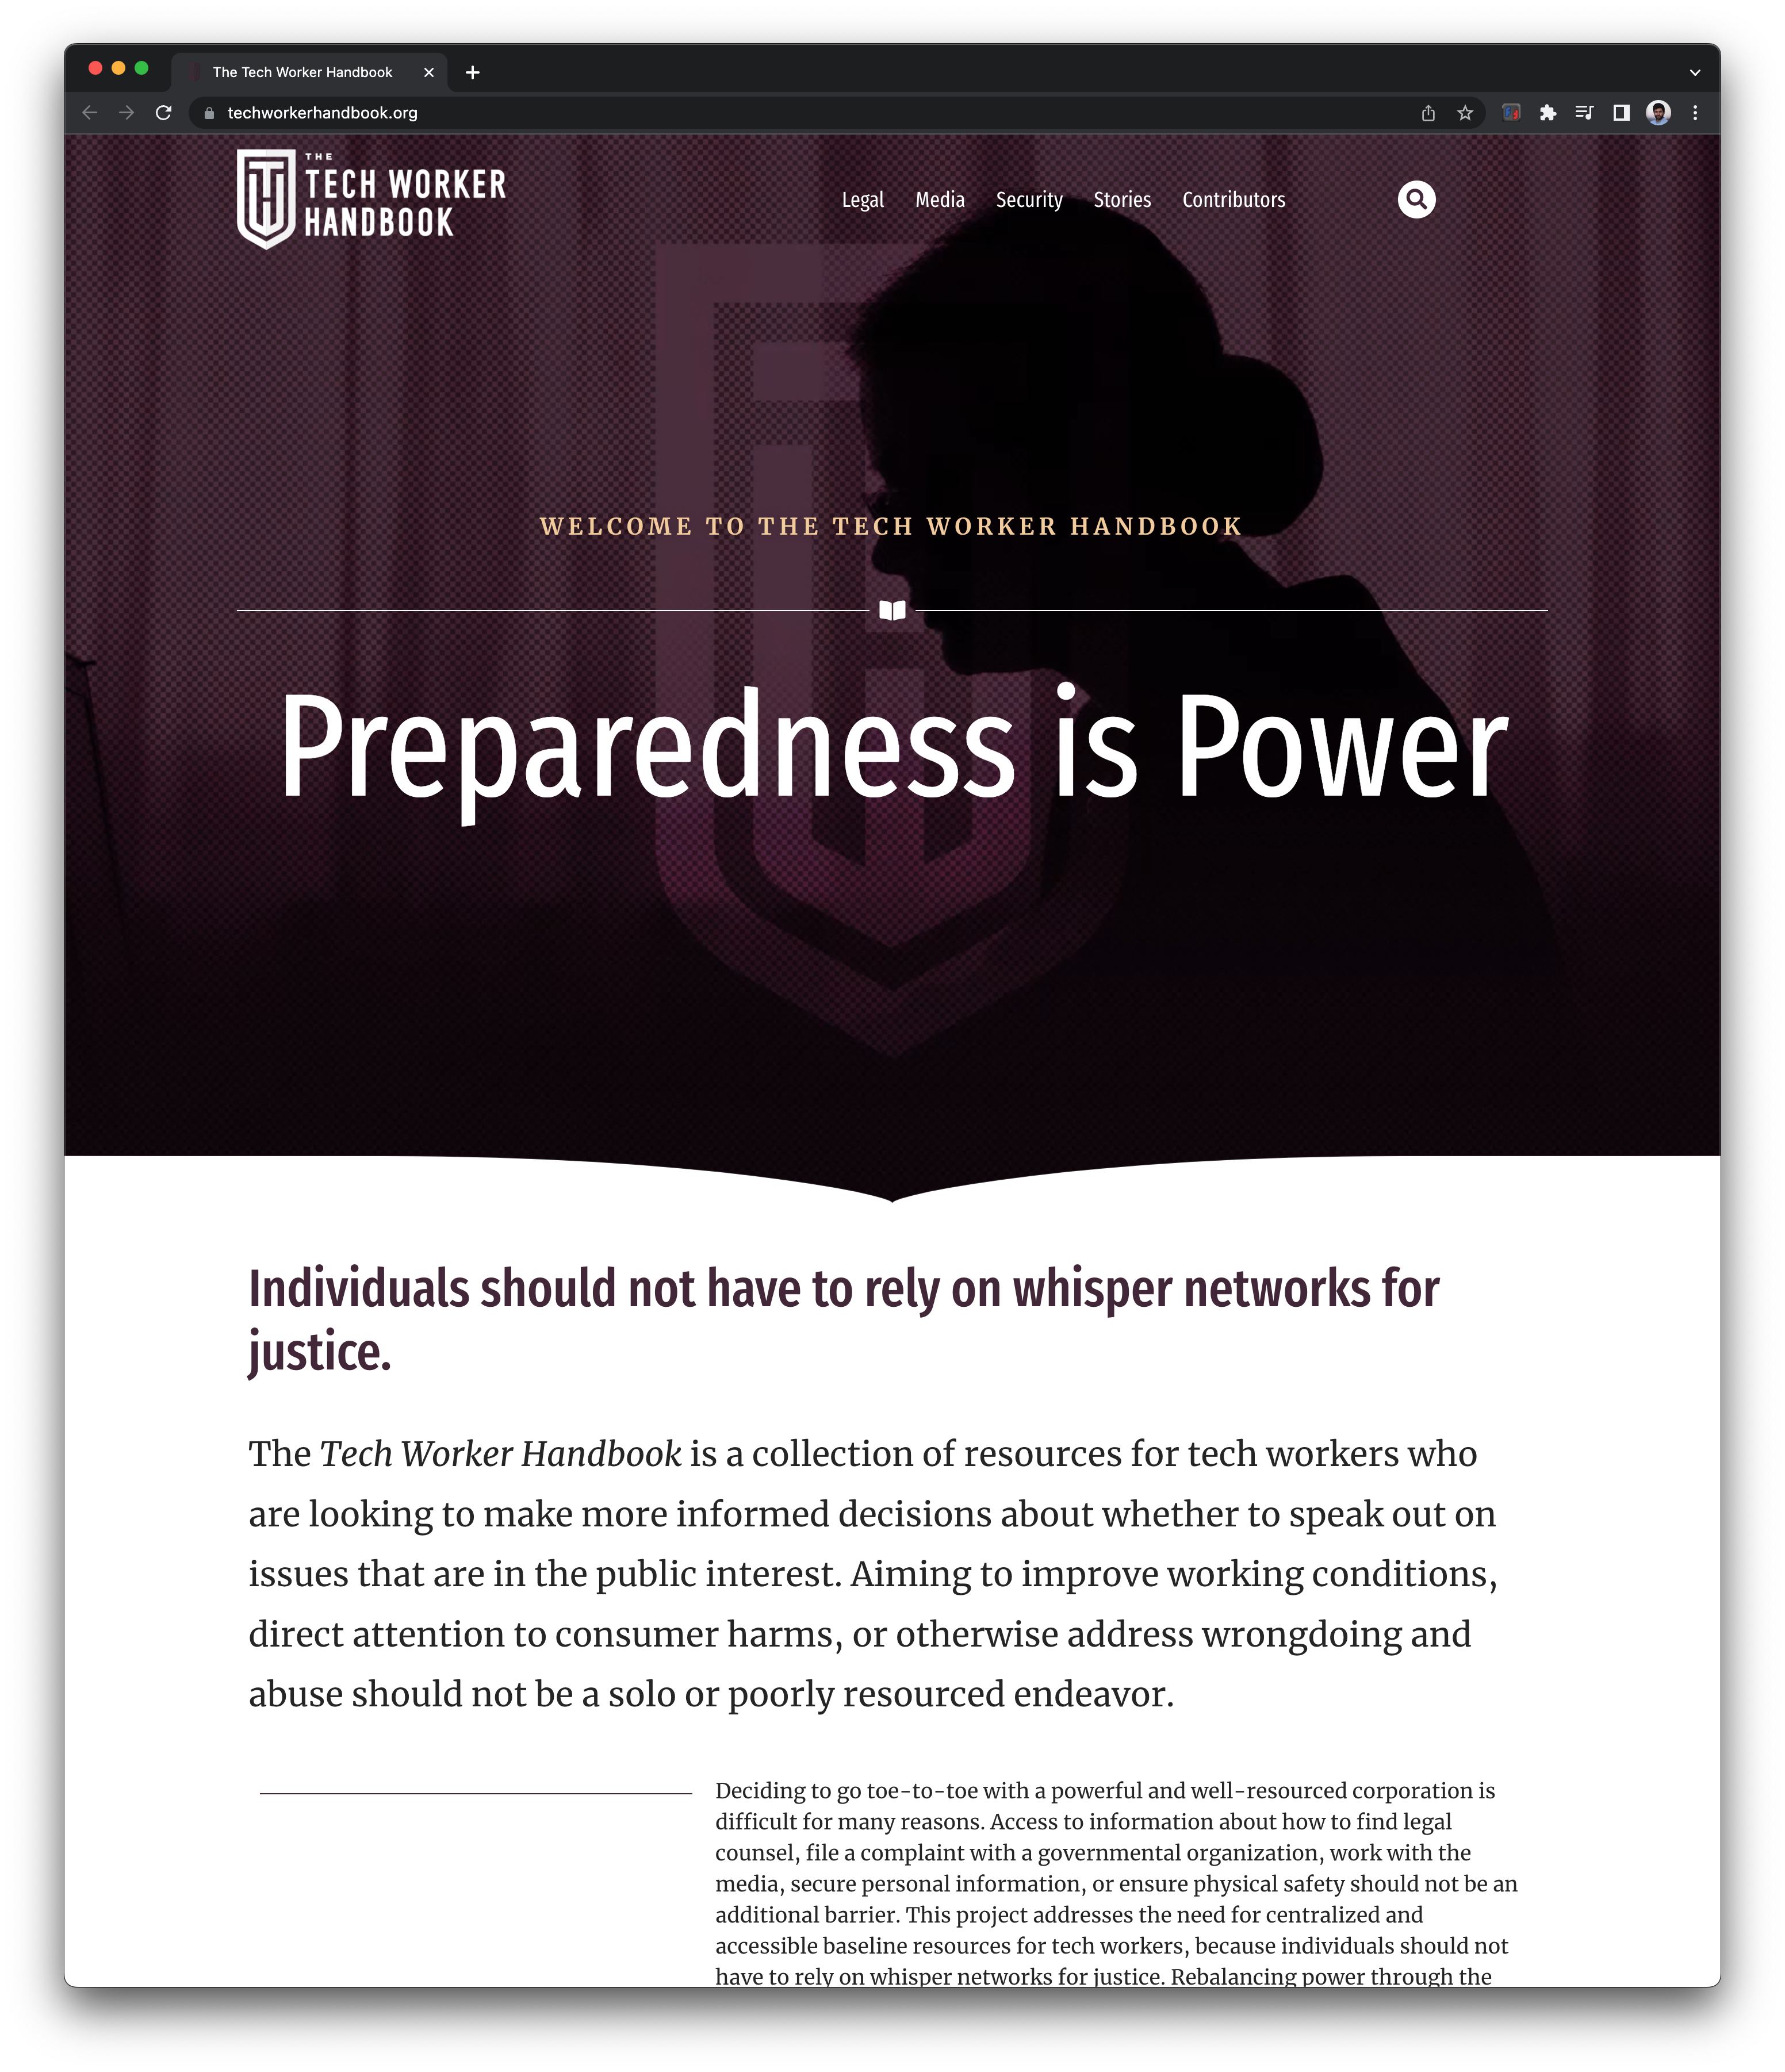
\includegraphics[width=1.5\textwidth]{figures/news/twh_2.png}

\end{column}
\end{columns}

\end{frame}




\begin{frame}[standout]

{why are we talking about non-disclosure agreements?}

\end{frame}

\begin{frame}[plain]
\centering

\only<+>{NDAs have routinely been used \\- \strong{especially in Silicon Valley} -\\ to prevent historically marginalized groups from discussing trauma they've experienced}

\only<+>{NDAs have also made it confusingly ambiguous what protections \\- \emph{if any} -\\ \strong{whistleblowers} have when they step forward with evidence of intentional or negligent harms}

\end{frame}

\begin{frame}{why does that matter?}

\visible<+->{We've discussed the importance of diverse teams.}

\visible<+->{We also need to understand the structural forces that make it difficult or impossible for people from historically marginalized backgrounds to continue to \emph{exist} in workplaces}


\end{frame}





\againframe<2>[plain]{newsythings}





\begin{frame}{Amazon Labor Union}
  
\begin{columns}
\begin{column}{0.7\textwidth}
\includegraphics[width=\textwidth]{figures/news/ALU.png}
\end{column}
\end{columns}
\end{frame}


\begin{frame}{Starbucks Labor Union}
  
\begin{columns}
\begin{column}{0.7\textwidth}
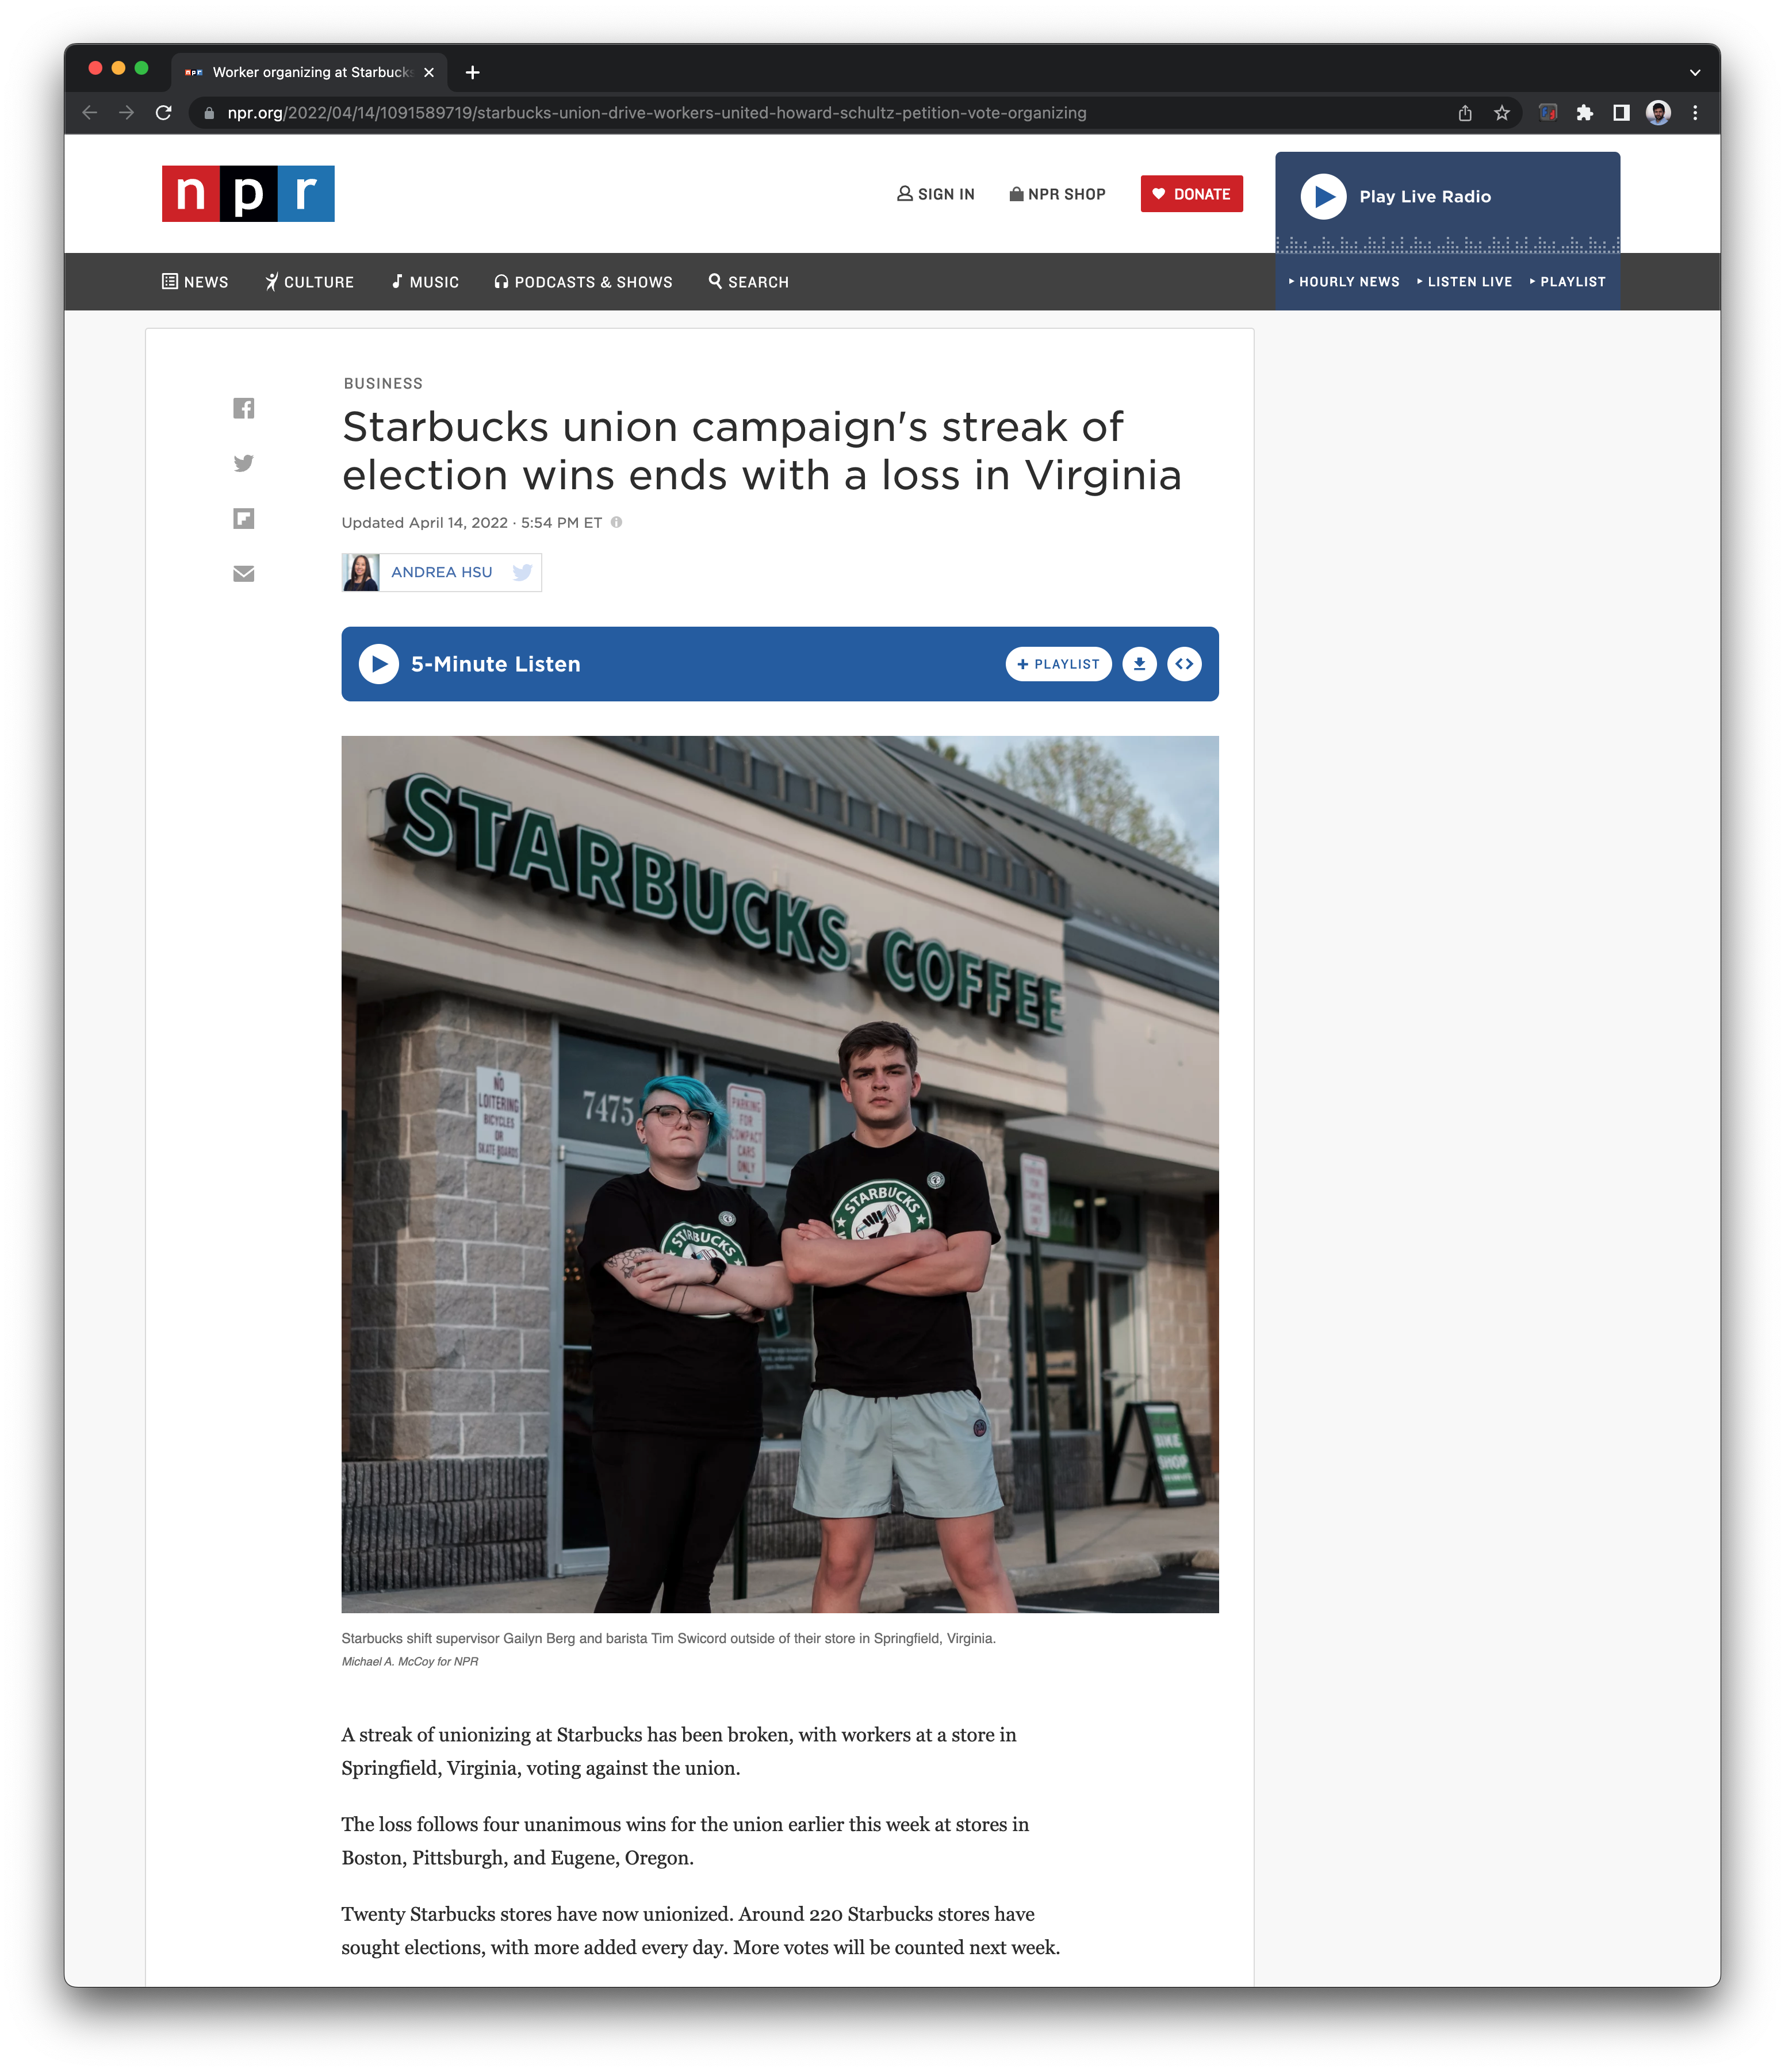
\includegraphics[width=\textwidth]{figures/news/SLU.png}
\end{column}
\end{columns}
\end{frame}


\begin{frame}{what can we learn?}
    
\begin{itemize}
  \item<+-> Open discussions about workplace conditions are good
  \item<+-> No corporation is too big to organize against
  \item<+-> You don't have to start big
\end{itemize}

\end{frame}



\begin{frame}{organizing}
    
\begin{itemize}
  \item community organizing
  \item workplace organizing
\end{itemize}

\end{frame}



\begin{frame}{questions?}
    This is probably the last chance to ask major content questions.

    Let's chat about whatever you want?

\end{frame}














\end{document}